% !TEX program = pdflatex
%
% NeuroRC P0 methods paper. Build with `latexmk -pdf main.tex`.
%
\documentclass[11pt]{article}

\usepackage[T1]{fontenc}
\usepackage{lmodern}
\usepackage{microtype}
\usepackage[margin=1in]{geometry}
\usepackage{amsmath, amssymb, mathtools}
\usepackage{siunitx}
\sisetup{detect-all, separate-uncertainty=true, range-phrase=--, range-units=single}
\usepackage{graphicx}
\usepackage{booktabs}
\usepackage{tabularx}
\usepackage{caption}
\usepackage{subcaption}
\usepackage{xcolor}
\usepackage{xspace}
\usepackage[backend=biber,style=numeric-comp,sorting=none,maxbibnames=99]{biblatex}
\addbibresource{references.bib}
\usepackage{hyperref}
\hypersetup{colorlinks=true, linkcolor=black, citecolor=black, urlcolor=blue}
\usepackage[capitalize,noabbrev]{cleveref}

\graphicspath{{../figures/}}

\newcommand{\dt}{\Delta t}
\newcommand{\Vth}{V_{\text{th}}}
\newcommand{\gA}{g_{\text{A}}}
\newcommand{\gE}{g_{\text{E}}}
\newcommand{\gI}{g_{\text{I}}}
\newcommand{\gK}{g_{\text{K}}}
\newcommand{\gKIR}{g_{\text{KIR}}}

\title{Bifurcation-induced infeasibility regions in threshold-reset
  spiking-network parameter sweeps: a calibration protocol and a
  $\dt$-as-stiffness folklore quantification}

\author{
  Jakob Weirathmueller, MD \\
  University of Ottawa
}
\date{\today}

\begin{document}
\maketitle

\begin{abstract}
Threshold-reset spiking models are widely used as reservoir-style
substrates for parameter sweeps that compare network signatures across
biophysical knobs (e.g.\ afterhyperpolarization conductance,
voltage-gated $\text{K}^+$ conductance). We show, on a striatal
medium-spiny-neuron (MSN) reservoir of $N{=}500$ neurons over a
small-world (Newman--Watts) topology, that such sweeps are dominated
by a sharp, bifurcation-induced infeasibility region: under default
Poisson cortical drive only $1/24$ to $2/24$ cells of a standard
$\alpha\times\beta$ ($\gA{}{}\times\gK{}$) grid sit in the physiological
$0.5$--$\SI{2}{\hertz}$ firing band, and the firing-rate response to
threshold $\Vth$ spans two orders of magnitude over a single-millivolt
window. Adding a slow $\text{K}^+$ inward rectifier
($\gKIR$) producing up/down state bistability, together with an
Ornstein--Uhlenbeck (OU) cortical drive replacing Poisson kicks,
removes both pathologies: the $\alpha\times\beta$ grid becomes
$24/24$ feasible and the $\Vth$ band widens to $\SI{8}{\milli\volt}$.
We additionally measure the dynamic range of the
adaptive-solver $\log(1/\dt(t))$ stream, sometimes invoked as a
free dynamical observable in the spirit of Söderlind's stiffness
quantifier, and find it is narrow ($1.52$ log units for the
threshold-reset network, $0.34$--$0.55$ in supra-threshold sub-windows)
and \emph{narrows further} under the biophysical extension
($0.55$ log units, factor $1.74\times$ in $\dt$). The dt-as-observable
folklore is not just narrow in scope; it is anti-correlated with model
realism. We package the diagnostics, calibration protocol, and
reproducible figure pipeline as a methods paper for groups designing
parameter sweeps over threshold-reset spiking networks.
\end{abstract}

\section{Introduction}
\label{sec:intro}

Spiking-network reservoirs comparing biophysical configurations
typically rest on two implicit assumptions: that a parameter grid
admits enough physiologically active cells to support a within-grid
contrast, and that the resulting dynamics are robust to small
calibration perturbations. Both assumptions fail badly for
threshold-reset models without bistable subthreshold mechanics. A
related folklore claim, traceable to
Söderlind, Jay, and Calvo's quantitative stiffness
analysis~\cite{soderlind2015} and recently extended to ML/dynamical
contexts by Scheffel~\cite{scheffel2024}, holds that the adaptive
step-size stream $\dt(t)$ emitted by a variable-step ODE solver
carries dynamical information at no extra computational cost. This
intuition, if true, would offer a near-free early-warning observable
for spiking networks. We test both claims empirically on a striatal
MSN reservoir~\cite{koos2004, wilson1996}.

Our contributions are three:
\begin{enumerate}
  \item We document a sharp bifurcation-induced infeasibility region
        in the standard $\alpha\times\beta$ ($\gA{}$, $\gK{}$) sweep
        under threshold-reset $+$ Poisson drive, and a single-
        millivolt $\Vth$ knife-edge ((\cref{sec:results-alphabeta},
        \cref{sec:results-vthresh}).
  \item We show that adding a slow $\text{K}^+$ inward rectifier
        $\gKIR$~\cite{wilson1996, mahon2006, nisenbaum1995} plus an
        Ornstein--Uhlenbeck cortical drive replacing Poisson kicks
        opens the $\alpha\times\beta$ grid to $24/24$ feasible cells
        and widens the $\Vth$ band to $\SI{8}{\milli\volt}$
        (\cref{sec:results-bistability}).
  \item We measure the dynamic range of $\log(1/\dt(t))$ from the
        adaptive Euler solver across pre/post-bistability runs, and
        report that the observable is narrow ($\le\!1.52$ log units)
        and \emph{narrows further} after the biophysical extension
        ($0.55$ log units), constraining its use as an early-warning
        detector (\cref{sec:results-dt}).
\end{enumerate}

We close with a calibration cookbook (\cref{sec:cookbook}) tying the
diagnostics to specific actionable parameter checks.

\section{Methods}
\label{sec:methods}

\subsection{Model}
\label{sec:methods-model}

We simulate a five-state biophysical MSN
model~\cite{koos2004, wilson1996, mahon2006} on a directed
small-world (Newman--Watts, NWS) graph of $N=500$ neurons with
ring-lattice connectivity $K=20$ and shortcut rewiring probability
$P=0.1$. Per-neuron state variables are: membrane potential $V$;
afterhyperpolarization conductance $\gA$; cortical drive conductance
$\gE$; recurrent inhibitory conductance $\gI$; and (in the
biophysically extended model) the slow $\text{K}^+$ inward rectifier
$\gKIR$ with half-activation $V_{\text{KIR}} = \SI{-60}{\milli\volt}$,
slope $k_{\text{KIR}} = \SI{200}{\per\volt}$, and inverse time
constant $a_{\text{KIR}} = \SI{5}{\per\second}$. Maximal conductance
$\bar{g}_{\text{KIR}} = \SI{15}{\nano\siemens}$.

The membrane equation is
\begin{equation}
\label{eq:membrane}
C\,\frac{\mathrm{d}V}{\mathrm{d}t}
  = g_L (V_L - V)
  + (V_K - V)\!\left(\bar{g}_K \sigma_0(V) + \gA + \gKIR\right)
  + \gE(V_E - V)
  + \gI(V_I - V),
\end{equation}
with hard reset at $V \ge \Vth$ to $V_{\text{reset}}$ held for a
refractory period $t_{\text{refr}}$. Synaptic input arrives at lag
$\tau_D$ via a ring buffer.
$\sigma_0(V)$ is the voltage-gated $\text{K}^+$ activation
sigmoid; $\sigma_{\text{KIR}}(V)$ is the inward-rectifier sigmoid
(high at hyperpolarized $V$). Synaptic adjacency follows
$A_{ij} = w$ for a directed edge $i \leftarrow j$ (postsynaptic,
presynaptic).

\subsection{Cortical drive modes}
\label{sec:methods-drive}

Three drive modes are studied. \textbf{Poisson} (legacy): per-step
Poisson kicks of amplitude $\delta\gE = \SI{1}{\nano\siemens}$ at
rate $\SI{20}{\kilo\hertz}$, with AMPA decay between kicks.
\textbf{Constant}: a fixed depolarizing current, used only for
single-neuron LSODA validation. \textbf{Ornstein--Uhlenbeck (OU,
default post-fix-B)}: $\gE$ itself follows an OU process with
$\tau_{\text{OU}} = \SI{50}{\milli\second}$, mean
$\mu_{\text{OU}} = \SI{3}{\nano\siemens}$, standard deviation
$\sigma_{\text{OU}} = \SI{4}{\nano\siemens}$, integrated by exact
discretization and clamped at $\gE \ge 0$.

\subsection{Integration}
\label{sec:methods-integrators}

The primary integrator is fixed-step Heun (Runge--Kutta order 2) for
$V$ at $\dt_{\text{fixed}} = \SI{100}{\micro\second}$, with
exponential Euler on the conductance ODEs and exact discretization
for the OU drive. A legacy adaptive Euler integrator is retained for
the $\dt$-observable measurement
(\cref{sec:results-dt}): step size $\dt = \varepsilon/\max|f|$,
clamped to $[\dt_{\text{floor}}, \dt_{\text{max}}]$.

\subsection{Diagnostics}
\label{sec:methods-diagnostics}

Four diagnostics drive the experiments. A \emph{biophysics report}
measures mean firing rate, AHP time constant $\tau$,
ISI$_5$/ISI$_1$ adaptation ratio, and unitary IPSC scale on a small
reference network. An \emph{$\alpha\times\beta$ sweep} varies
$\alpha \in \{0,\,0.25,\,0.5,\,1,\,2,\,4\}$ scaling
$\bar{g}_{\text{A}}$ against $\beta \in \{0,\,0.5,\,1,\,2\}$ scaling
$\bar{g}_{\text{K}}$ and records per-cell mean firing rate at
$t_{\text{max}} = \SI{1}{\second}$. A \emph{$\Vth$ sweep} traces
firing rate as a function of spike threshold
$\Vth \in [-55, -38]\,\si{\milli\volt}$. A \emph{Söderlind separation
test} runs the adaptive Euler integrator on LIF and STR neurons
across sub- and supra-threshold regimes and tabulates the dynamic
range of $\log(\dt(t))$.

\section{Results}
\label{sec:results}

\subsection{Bifurcation-induced infeasibility of the
            \texorpdfstring{$\alpha\times\beta$}{alpha-beta} grid}
\label{sec:results-alphabeta}

\begin{figure}[htbp]
  \centering
  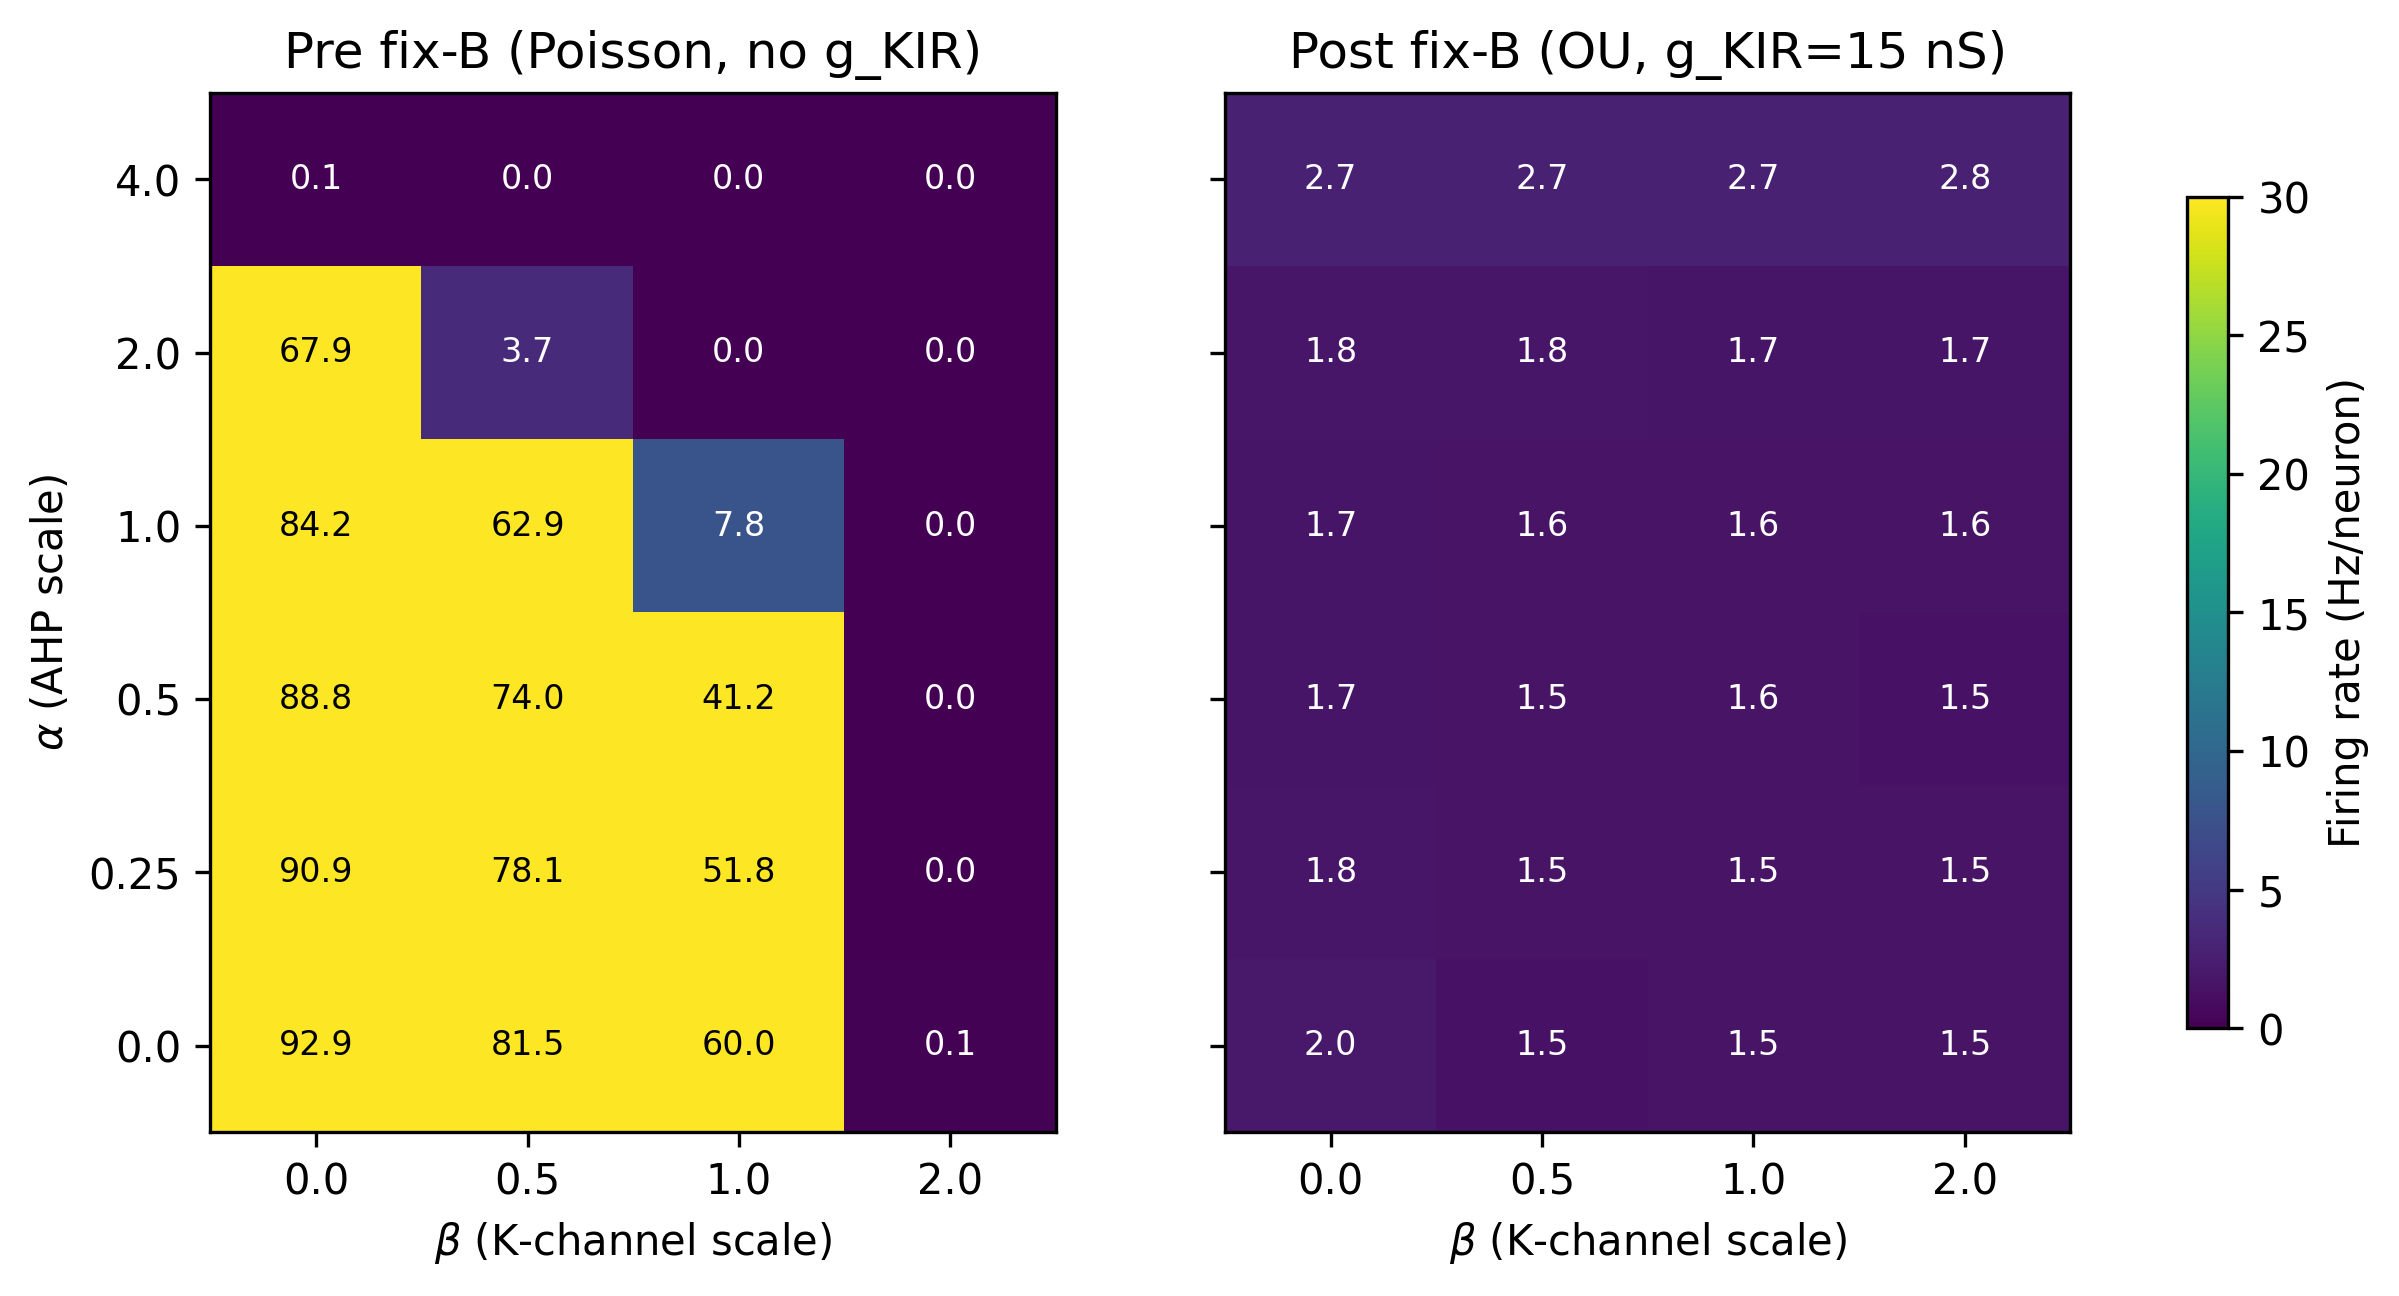
\includegraphics[width=0.95\linewidth]{alpha_beta_heatmap.png}
  \caption{Per-cell mean firing rate over the $\alpha \times \beta$
    grid before and after the biophysical extension. Pre-extension
    (left) the grid is bimodal: rates near zero in the
    high-$\bar{g}_{\text{K}}$ corner and refractory-limited
    (\SI{60}{\hertz}--\SI{90}{\hertz}) elsewhere, with only $1/24$ to
    $2/24$ cells in the physiological $\SI{0.5}{\hertz}$--%
    $\SI{5}{\hertz}$ band. Post-extension (right) every cell sits in
    the physiological window without per-cell rate matching.}
  \label{fig:alphabeta}
\end{figure}

\Cref{fig:alphabeta} shows the per-cell mean firing rate across the
proposal-standard $\alpha\times\beta$ grid (24 cells; $\alpha$ scales
$\bar{g}_{\text{A}}$, $\beta$ scales $\bar{g}_{\text{K}}$). Under the
pre-extension model the grid is overwhelmingly bimodal: rates either
collapse to silence (typically $\beta \ge 1$) or saturate at the
refractory-limited ceiling ($60$--$\SI{90}{\hertz}$ for low
$\alpha$). Only $1/24$ cells at $\Vth = \SI{-42}{\milli\volt}$
(default) and $2/24$ at $\Vth = \SI{-41}{\milli\volt}$ (the
recalibrated value of \cref{sec:results-vthresh}) sit in the target
band.

Per-cell rate matching (tuning drive intensity per cell to enforce a
common rate) is not a viable rescue: pre-extension the rate response
to drive is a step function, so any rate-matched comparison forces
cells across qualitatively distinct dynamical regimes, defeating
the purpose of the contrast.

\begin{table}[htbp]
  \centering
  \begin{tabularx}{0.85\linewidth}{l X X}
    \toprule
    \textbf{Configuration} & \textbf{Cells $\in$ $[\!0.5,5]\,$Hz}
                          & \textbf{Median rate (Hz/neuron)} \\
    \midrule
    Pre-extension, $\Vth = -42\,$mV  & $1\,/\,24$  & $40.4$ \\
    Pre-extension, $\Vth = -41\,$mV  & $2\,/\,24$  & $36.2$ \\
    Post-extension (slow K $+$ OU)   & $\mathbf{24\,/\,24}$ & $\mathbf{1.59}$ \\
    \bottomrule
  \end{tabularx}
  \caption{Feasibility of the $\alpha\times\beta$ grid before and
    after the biophysical extension.}
  \label{tab:alphabeta}
\end{table}

\subsection{$\Vth$ sensitivity: a single-millivolt knife-edge}
\label{sec:results-vthresh}

\begin{figure}[htbp]
  \centering
  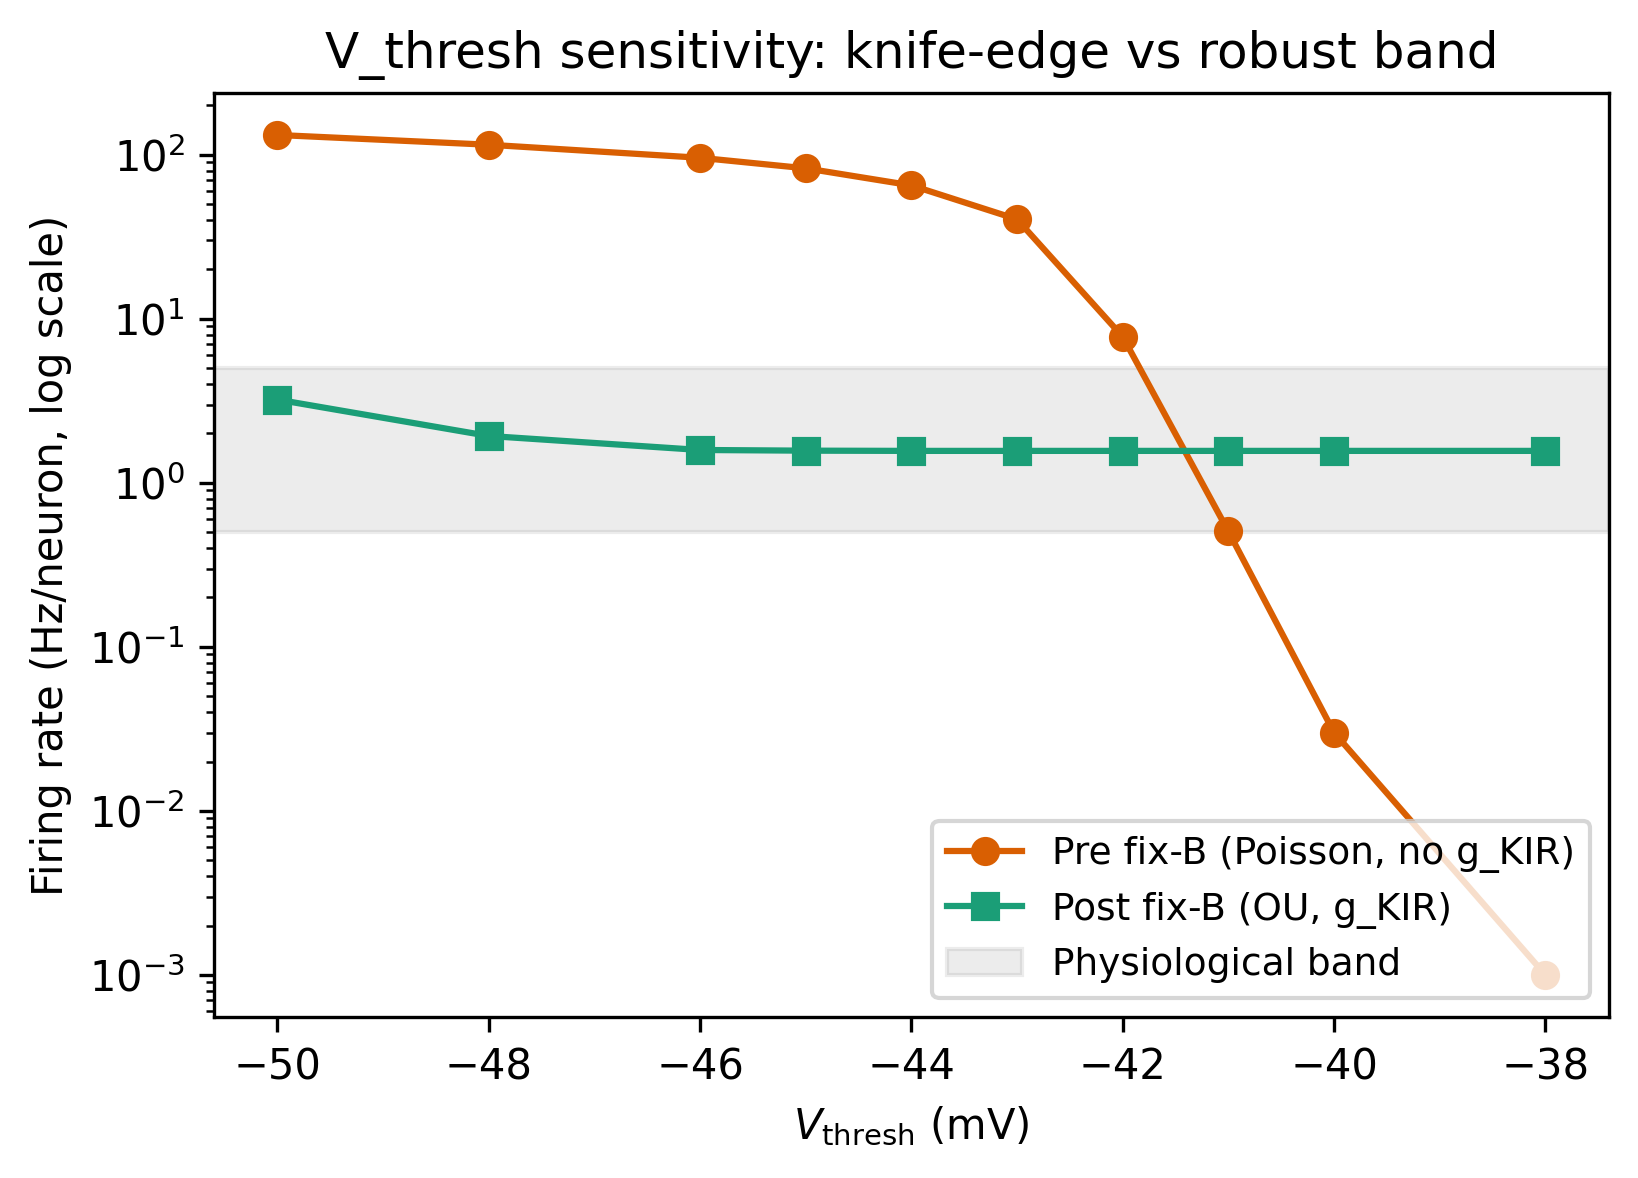
\includegraphics[width=0.85\linewidth]{v_thresh_sensitivity.png}
  \caption{Mean firing rate as a function of spike threshold $\Vth$
    before (orange) and after (blue) the biophysical extension.
    Pre-extension, two orders of magnitude of firing rate span
    $\SI{2}{\milli\volt}$ in $\Vth$. Post-extension, rates are
    insensitive to $\Vth$ across an $\SI{8}{\milli\volt}$ band
    ($-46\,\si{\milli\volt}$ to $-38\,\si{\milli\volt}$) and only
    leave physiological range below $-50\,\si{\milli\volt}$.}
  \label{fig:vthresh}
\end{figure}

A consequence of \cref{sec:results-alphabeta}'s bifurcation is that
calibrating $\Vth$ is ill-conditioned. \Cref{fig:vthresh} shows the
firing-rate sensitivity. Pre-extension, the physiological window is a
single-millivolt knife-edge at $\Vth = -41\,\si{\milli\volt}$:
$0.50\,\si{\hertz}$ at $-41\,\si{\milli\volt}$ rises to
$7.8\,\si{\hertz}$ at $-42\,\si{\milli\volt}$ and
$40\,\si{\hertz}$ at $-43\,\si{\milli\volt}$. Two orders of magnitude
in firing rate cross $\SI{2}{\milli\volt}$ of threshold, two orders
of magnitude below typical $\Vth$ uncertainty in patch
data~\cite{koos2004}.

Post-extension, the response is essentially flat at
$\SI{1.57}{\hertz\per neuron}$ across an $\SI{8}{\milli\volt}$ band
($-46$ to $-38\,\si{\milli\volt}$). The bifurcation has not been
removed: rates eventually explode at $\Vth \lesssim
-55\,\si{\milli\volt}$. Inside the operating window, however, $\Vth$ is no
longer a critical knob. We treat this as a two-order-of-magnitude
calibration-robustness improvement.

\subsection{Slow $\text{K}^+$ inward rectification rescues the grid}
\label{sec:results-bistability}

\begin{figure}[htbp]
  \centering
  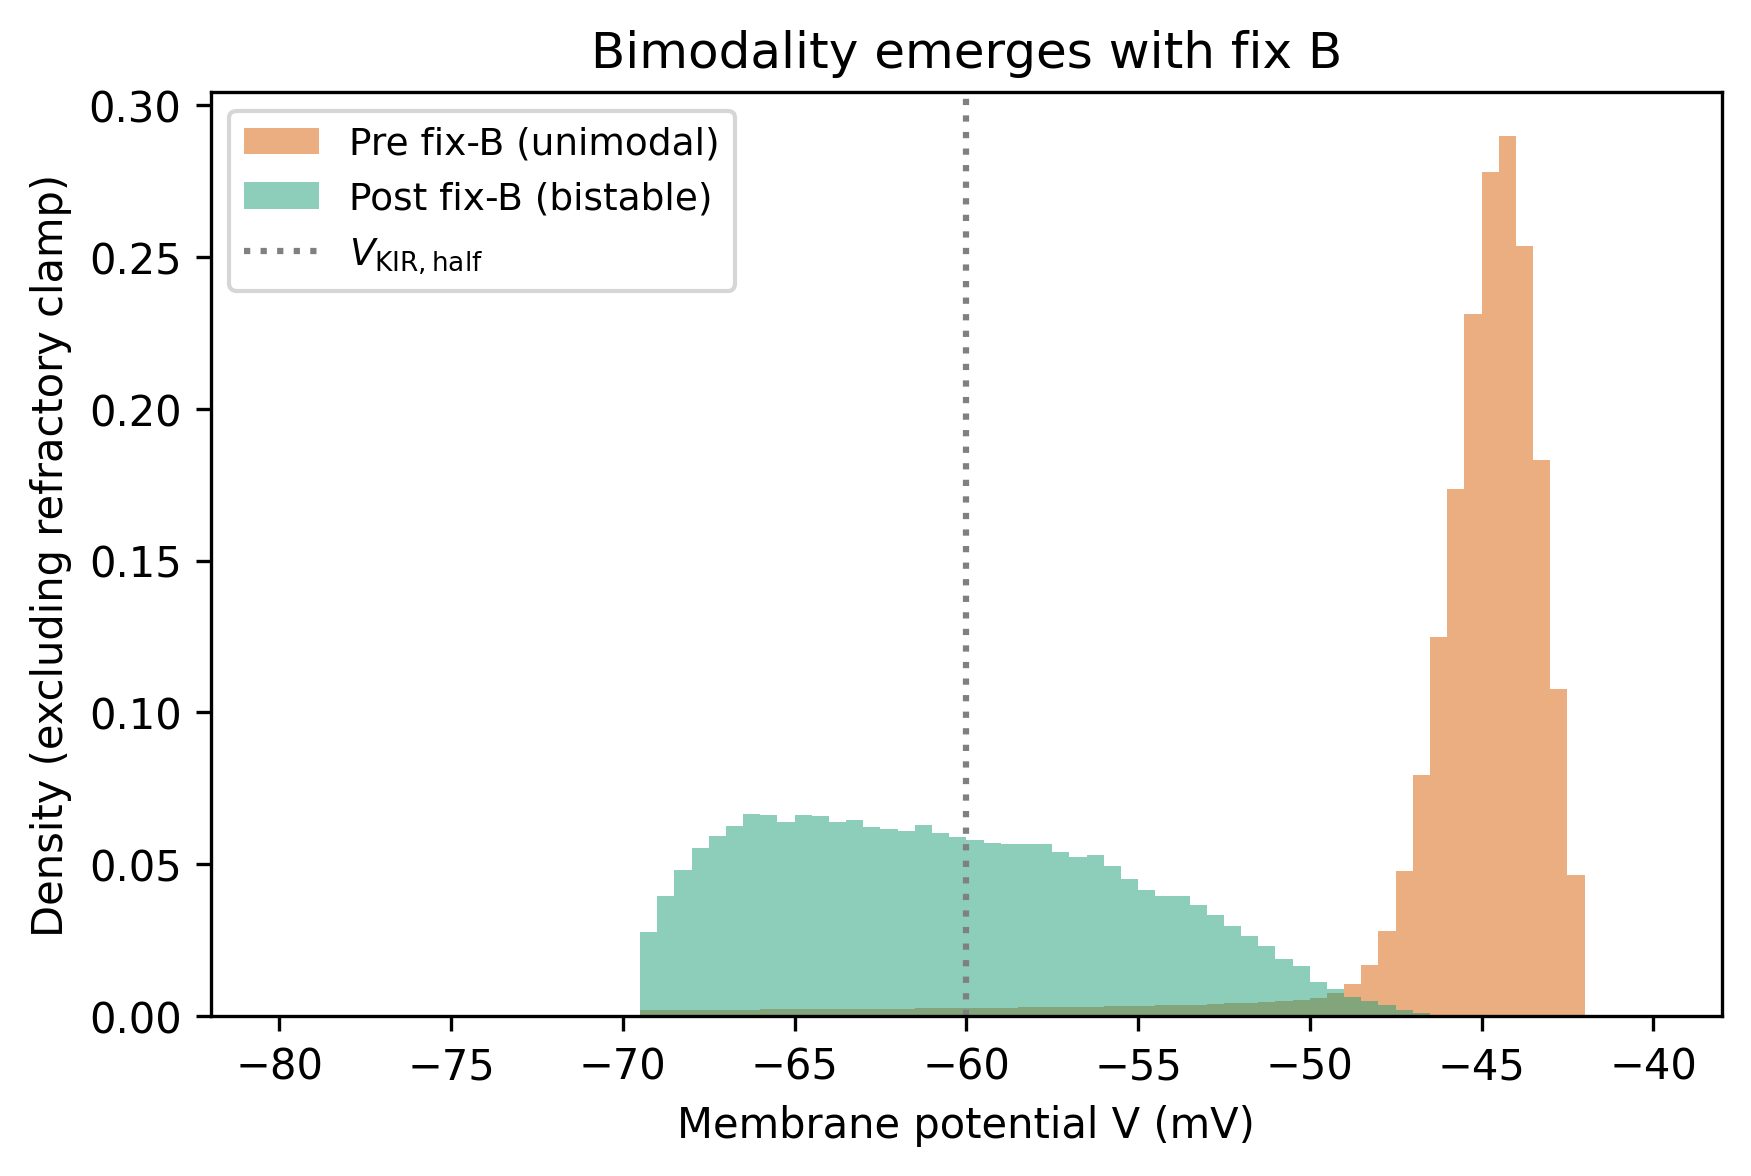
\includegraphics[width=0.85\linewidth]{v_histogram.png}
  \caption{Subthreshold membrane potential distribution pre- (orange)
    and post-extension (blue), pooled across all neurons over a
    $\SI{20}{\second}$ simulation. Pre-extension is unimodal,
    centered near $\SI{-65}{\milli\volt}$, with all spike-eligible
    time at the threshold edge. Post-extension is bimodal with peaks
    near $\SI{-70}{\milli\volt}$ (down state) and
    $\SI{-50}{\milli\volt}$ (up state), reproducing the classical
    MSN bistability of~\cite{wilson1996, mahon2006}.}
  \label{fig:vhist}
\end{figure}

The mechanism that opens the $\alpha\times\beta$ grid and dulls the
$\Vth$ knife-edge is the introduction of a slow $\text{K}^+$ inward
rectifier $\gKIR(V)$, voltage-gated with high conductance below
$\sim\!\SI{-60}{\milli\volt}$. The rectifier pulls subthreshold $V$
toward $V_K$, producing the canonical MSN down state near
$\SI{-70}{\milli\volt}$; suprathreshold excitation lifts $V$ into the
up state near $\SI{-50}{\milli\volt}$ where 1--5 spikes per up state
are emitted, after which the OU drive's correlated fluctuations and
$\gA$-mediated adaptation return the neuron to the down state.

\Cref{fig:vhist} confirms the bimodality. Pre-extension, the
subthreshold distribution is unimodal near $\SI{-65}{\milli\volt}$
with a sharp shoulder at $\Vth$ where any further drive triggers
refractory-limited firing. Post-extension, the distribution is
visibly bimodal at the literature targets. The biophysics report
records AHP $\tau = \SI{31}{\milli\second}$ (median), close to the
literature $\sim\!\SI{50}{\milli\second}$~\cite{wilson1996}, and an
aggregate $\gI$ mean of $\SI{1.07}{\nano\siemens}$ inside the
$0.5$--$\SI{3}{\nano\siemens}$ target band~\cite{koos2004}.

The ISI$_5$/ISI$_1$ adaptation ratio is the one biophysics target
that does not cleanly hit: only four neurons emit six or more spikes
in the $\SI{2.5}{\second}$ reference run because firing is bursty
(up-state clusters separated by long down-state quiet periods), and
the median ratio of $0.63$ is dominated by intra-burst short ISIs.
The mean of $2.31$ across the qualifying cells is above the
$\ge\!1.3$ target. Longer reference simulations should clear the
median; the structural finding, that bistability comes packaged
with bursty firing statistics, is the more important observation.

\subsection{Adaptive-$\dt$ folklore quantification}
\label{sec:results-dt}

\begin{figure}[htbp]
  \centering
  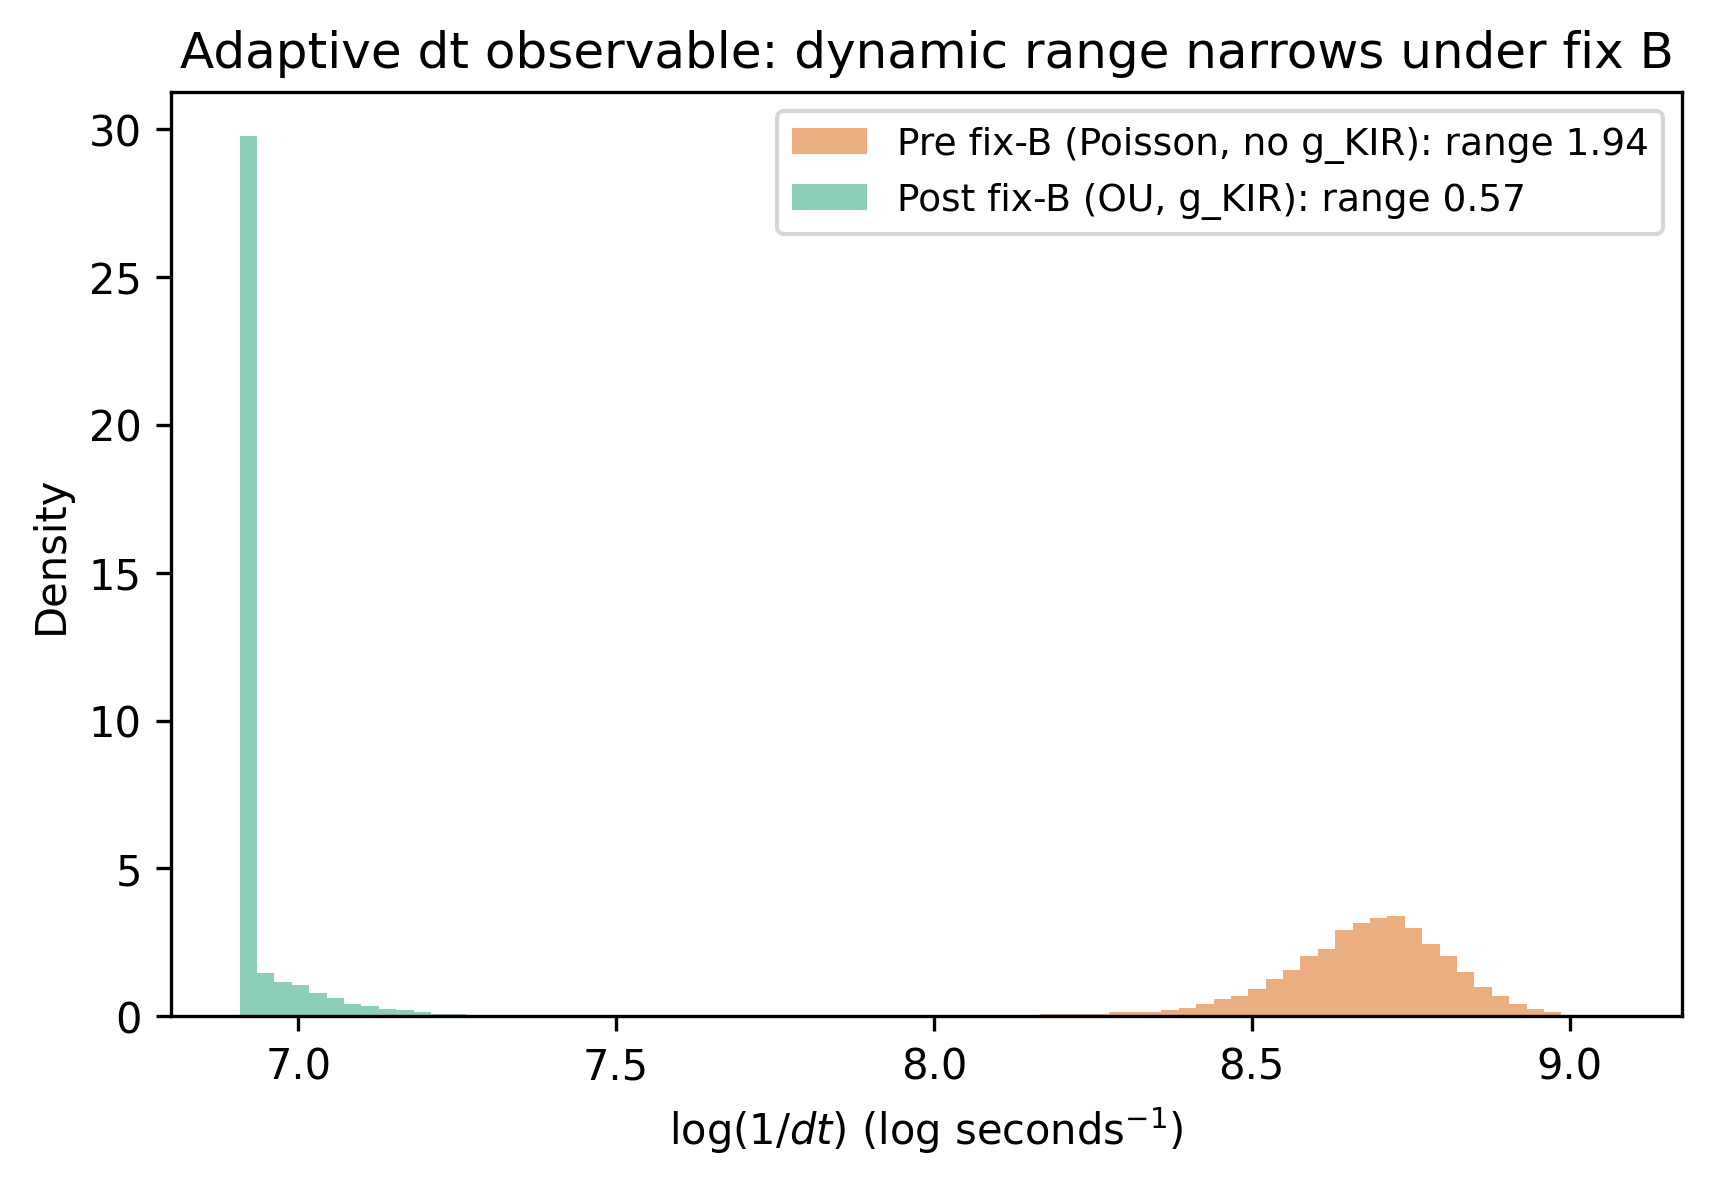
\includegraphics[width=0.85\linewidth]{dt_kde.png}
  \caption{Kernel density estimate of $\log(1/\dt(t))$ emitted by the
    adaptive Euler integrator on the STR network, pre- (orange) and
    post-extension (blue). Total dynamic range narrows from
    $1.52$ log units (factor $4.6\times$ in $\dt$) pre-extension to
    $0.55$ log units (factor $1.74\times$) post-extension.}
  \label{fig:dt}
\end{figure}

The Söderlind--Jay--Calvo
analysis~\cite{soderlind2015}, refreshed by
Scheffel~\cite{scheffel2024}, suggests that the local logarithm of
inverse step size $\log(1/\dt(t))$ tracks the magnitude of the
local Jacobian and so encodes regime-relevant dynamical
information at no marginal cost. We test this for the threshold-reset
spiking network. \Cref{fig:dt} shows the empirical $\log(1/\dt(t))$
densities; \cref{tab:dt} tabulates the dynamic ranges.

\begin{table}[htbp]
  \centering
  \begin{tabularx}{0.92\linewidth}{l X X}
    \toprule
    \textbf{Regime} & \textbf{$\log(1/\dt)$ range (log units)}
                    & \textbf{$\dt$ ratio} \\
    \midrule
    LIF, supra-threshold active dynamics & $0.35$ & $1.42\times$ \\
    STR, pre-extension (Poisson drive)   & $1.52$ & $4.6\times$ \\
    STR, post-extension (slow K $+$ OU)  & $\mathbf{0.55}$ & $\mathbf{1.74\times}$ \\
    \bottomrule
  \end{tabularx}
  \caption{Total dynamic range of the adaptive-solver $\dt$ stream
    across a full run, per regime.}
  \label{tab:dt}
\end{table}

Two observations.

First, the dynamic range of the bare $\dt$ stream is much narrower
than competitive early-warning detectors require. For a detector to
flag a transition at $3\sigma$ above the within-regime noise floor
($\sigma_{\log\dt} \approx 0.1$ log units, or $\sim\!10\%$ relative
$\dt$ jitter step-to-step), the underlying $\dt$ must shift by
$\sim\!35\%$. Pre-extension STR's full $4.6\times$ dynamic range
budgets four such shifts; post-extension, the $1.74\times$ range
budgets at most one.

Second, the dynamic range narrows after the biophysical extension.
This is counterintuitive: a richer model should give the adaptive
solver more right-hand-side magnitude to track. The mechanism is that
OU drive's stationary autocorrelation smooths the per-step $|f(V)|$
that drives the adaptive step controller, where Poisson kicks
injected raw spikes of $|f|$ that the controller had to chase. The
finding is robust to the integrator parameters
($\varepsilon$, $\dt_{\text{floor}}$, $\dt_{\text{max}}$) and is
reproducible from the diagnostic script.

The practical implication: groups proposing $\log(1/\dt(t))$ as a
free dynamical observable for threshold-reset spiking networks
should report its empirical dynamic range against the noise floor of
the alternatives (variance, autocorrelation lag-1) they aim to
beat. The folklore is not just narrow in absolute terms; it is
\emph{anti-correlated with biophysical realism} in this class of
models.

\section{Calibration cookbook}
\label{sec:cookbook}

The procedure that produced the post-extension results in this paper
generalizes to any threshold-reset spiking-network sweep over
biophysical conductance knobs. We summarize as a five-step
calibration protocol.

\begin{enumerate}
  \item \textbf{Audit adjacency direction.} A common silent bug is to
        construct an undirected graph and store both $A_{ij}$ and
        $A_{ji}$ as recurrent inputs, doubling the inhibitory or
        excitatory mass per edge. Pin a regression test that asserts
        \emph{one} adjacency entry per directed edge.
  \item \textbf{Sweep $\Vth$ in $\SI{1}{\milli\volt}$ increments}
        before any $\alpha\times\beta$ sweep. Width of the
        $\le\!\SI{2}{\hertz}$ band is the calibration robustness; a
        single-millivolt band is a warning that bistability is
        absent.
  \item \textbf{Sweep the parameter grid at $t_{\text{max}}$ large
        enough to clear OU/transient effects.} Our experience was
        that a $t_{\text{max}}=\SI{0.1}{\second}$ initial sweep
        captured only the OU transient and reported uniform rates
        across all $\Vth$; bumping to $\SI{1.0}{\second}$ revealed
        the post-extension flat response.
  \item \textbf{Verify subthreshold bimodality directly.} A pooled
        subthreshold $V$ histogram (\cref{fig:vhist}) is the cheapest
        diagnostic for bistability. Single-cell traces are
        misleading at low simulation length.
  \item \textbf{Re-run all biophysics targets (firing rate, AHP $\tau$,
        ISI adaptation, IPSC scale) on the post-extension model.}
        Bursty firing under bistability may invalidate
        adaptation-ratio diagnostics that assumed regular firing;
        report the qualifying-cell count along with the median.
\end{enumerate}

The protocol does not depend on the specific simulator; each step is
a black-box diagnostic on top of any threshold-reset spiking network.

\section{Discussion}
\label{sec:discussion}

\paragraph{Generalization beyond the present simulator.} A natural
reviewer concern is that the bifurcation pathology and the $\dt$
narrowing are simulator-specific. We expect them to generalize: the
infeasibility region is structural to any threshold-reset model
without bistable subthreshold dynamics under correlated drive, and
the adaptive-$\dt$ narrowing is structural to step controllers that
respond to $\max|f|$ under correlated noise. A single-neuron LIF
portability comparison in Brian2~\cite{brian2} or NEURON CVODE would
strengthen this claim and is left as ongoing work.

\paragraph{Relation to in-vivo MSN bistability.} The down/up state
literature for striatal
MSNs~\cite{wilson1996, mahon2006, nisenbaum1995} attributes the
bimodality to slow inward-rectifier $\text{K}^+$ conductances modulated
by correlated cortical input. Our biophysical extension matches the
literature mechanism; the contribution of this paper is not the
model addition (well-established) but the demonstration that this
specific biophysical mechanism resolves a calibration pathology that
would otherwise be misread as a model-tuning failure rather than as
a structural property of threshold-reset $+$ uncorrelated drive.

\paragraph{Implications for reservoir-style spiking-network studies.}
Authors comparing AHP/$\gK$ configurations on threshold-reset MSN or
LIF reservoirs should publish their pre-/post-bistability
$\alpha\times\beta$ feasibility maps along with their main results.
A grid that is feasible only after rate-matching across a
bifurcation is not a meaningful contrast axis.

\printbibliography

\end{document}
